\subsection{IN PROGRESS. Present consequences and outcomes}

To make a good selection in the dataset of the fields that are relevant or the combination of these, it is essential to
solid knowledge on the subject to be treated. Therefore, it is fundamental to dedicate the necessary time to enter the
importance of the concept, what benefits it can bring or what situations can dameage us.
The points that should be clear in the design phase are: \\

\textbf{Objective}. Conceptually, what problems do we want to solve or clarify. It is very important that we have a clear objective,
     Even if we do not have prior expertise in the subject, having a well-defined objective helps us find the solution, or
     at least enables us to describe it more clearly to the expert who can solve the problem. \\

\textbf{Important points. Notable situations}. As we mentioned earlier, our goal is not to show all the values, but
     which is about providing the user with important information in order to discover the significant situations that influence the
     us, either positive or negative. At a more technical level, it would be the limits or values of what data are those that provide us with information
     of an exceptional situation, or the values that we are trying to identify more easily. \\

\textbf{Data workflow}. When planning the flow of information, it must be clear how to get from one point to another. For example, 
we should start simple and move to more complex representations.

\subsubsection*{Suggested strategies} 

\begin{itemize}
    \item Once a goal has been set, we must stipulate the necessary fields of the dataset that we need. That is, we select the fields that interest us. 
    \item Following this, we need to analyze the data provided and see if the list of fields that the source offers us is sufficient to rech the chosen objective.
    If not directly, we the combination of them.
    \item Next, we decide which values are more outstanding and we will provide them to the user.
\end{itemize}

\subsubsection*{In the context of Aire Guru \ldots}

Our main objective is to create awareness of the importance of air pollution in our health. For this we investigate different concepts:

\begin{itemize}
    \item What diseases are affected by air pollution.
    \item What pollutants are those that create or influence diseases.
    \item What are the sources of each pollutant?.
    \item What is the representative measure of the level of air pollution.
    \item How it is calculated and what parameters we need for its calculation.
    \item What are the harmful levels in general and for each pollutant.
\end{itemize}

The measure that best represents the level of air pollution, in this case is the AQI. The city of Málaga is covered by the European legislation, 
so we focus investigations of official sources in this regulation.
We look for the relationships that pollutants have with different diseases, for this we resort to clinical studies. For each of the diseases, we 
research at the symptoms and how they can be aggravated by each pollutant.
For each pollutant, we look for sources of pollution and see if they occur in the city of Málaga and in what concentrations.
With all this information we define that the pollutants that affect air quality are CO, NO2, O3 and PM (Particulated Material). Dfferent levels of particles
affect different diseases in different ways. \\

As the main objective is awareness, we provide all the data in an organized way in the Glossary of Air Guru. \\

Once these pollutants are selected, we verify if we have the particular data in our dataset. As we mentioned earlier, some samples show measurements 
from fixed and / or mobile stations and these can be quantitative or qualitative and others can be incomplete. We will have to select the
samples to provide us with the most complete information or the most accurate, in this case the quantitative measure will prevail to the qualitative 
one and in the case that there is only qualitative
the following values are decided: Good: 50, Acceptable: 150, Poor: 300, Bad: 400, Unhealthy: 500 and the user will be informed when the value is qualitative. \\

At this point we know how air pollution affects our health, We make very clear which are the undesirable values by using the alert colors, yellow, orange and 
red. These colors are chosen in the palette of the colors provided by the EAQI.
Height is used in graphics, since it is an intuitive representation for humans. In addition, the icon that represents unhealthy levels of pollution, is
totally different, designed to clearly convey danger. \\

\begin{figure}[ht]
    \centering
    \subfigure[BarChart Aire Guru]
        {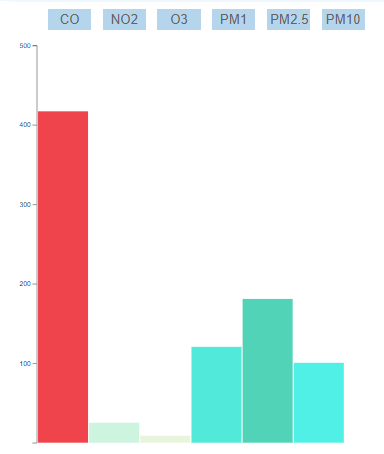
\includegraphics[width=5cm  ]{barchart}}
    \hfill
    \subfigure [Categoria medio ambiente]
        {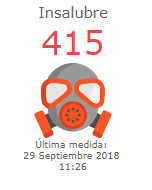
\includegraphics[width=4cm]{unhealthyIcon}}
    \caption{Alert situation}
\end{figure}

Regarding the workflow, we are guiding the user from the selection of a point in the city of Málaga, either on his own initiative
or automatic to the details of this point in real time and we continue to show  the evolution of the pollution at that point.
The logic of this development is that it is anticipated that the user will be interested in the pollution that surrounds him in real time and if
he wanta to know the breakdown of the pollutants at the point where he is, he can continue to inquire. The map, in addition to showing
the point where the user is, serves as verification, gives more realism and confidence to the user.

\begin{itemize}
    \item The objective has been clearly defined and an investigation has been carried out, determining if the dataset is appropriate.
    \item Worrying levels have been defined as poor, bad and unhealthy and are represented in the Air Guru website. They stand out clearly so that the user is able to locate them quickly.
    \item The workflow is satisfactory, since the user knows the level of pollution at any location, at a simple glance. It is easy to explore the information further, if the user wishes.
\end{itemize}